\chapter{Giới thiệu}
\label{Chapter1}

Các mạng nơ-ron nhiều tầng ẩn có tính ứng dụng cao và ảnh hưởng lớn tới ngành trí tuệ nhân tạo. Đầu tiên, các bài toán khó đối với máy tính như xử lý ảnh và ngôn ngữ tự nhiên đã phần nào được giải quyết. Thứ hai, các mô hình mạng nơ-ron có thể được sử dụng trong nhiều bài toán khác nhau, từ đó tăng tính ứng dụng vào thực tế. Thứ ba, các lý thuyết liên quan đến mạng nơ-ron nhiều tầng ẩn vẫn còn nhiều câu hỏi chưa có lời giải đáp, cho thấy tiềm năng của hướng phát triển này.

Mạng nơ-ron nhân tạo (Artificial Neural Network) gồm: tầng nhập, các tầng ẩn và tầng xuất. Mỗi tầng được cấu thành từ nhiều đơn vị tính toán mà ta gọi là các nơ-ron. Các nơ-ron được liên kết với nơ-ron ở tầng tiếp theo bằng các liên kết có trọng số đại diện cho mức độ quan trọng của tín hiệu từ nơ-ron này sang nơ-ron khác. Số lượng trọng số sẽ tăng theo số lượng tầng ẩn có trong mạng cũng như số lượng nơ-ron của mỗi tầng ẩn. Mạng nơ-ron nhân tạo có hơn một tầng ẩn được gọi là mạng nơ-ron nhiều tầng ẩn, hay mạng nơ-ron sâu (Deep Neural Network); ngược lại, gọi là mạng nơ-ron có ít tầng ẩn, hay mạng nơ-ron nông (Shallow Neural Network). Việc có nhiều tầng ẩn giúp mạng biểu diễn được các hàm phức tạp mà các mô hình học máy truyền thống không biểu diễn được. Ngoài ra, mạng học sâu còn có thể biểu diễn được cùng một tập hàm nhưng với số lượng trọng số ít hơn mạng nơ-ron nông \cite{bengio2009learning}. Sức mạnh rút trích đặc trưng tự động của mạng nơ-ron nhiều tầng ẩn đã được chỉ ra trong nhiều bài báo khác: Yoshua Bengio và Yann LeCun lý giải rằng với nhiều tầng ẩn, mạng nơ-ron có thể ``học'' được từ đặc trưng đơn giản (low-level features) và tạo thành các đặc trưng phức tạp hơn (higher-level features) (hình \ref{fig:layers-features}) \cite{bengio2007scaling}.

\begin{figure}[htp]
	\centering
	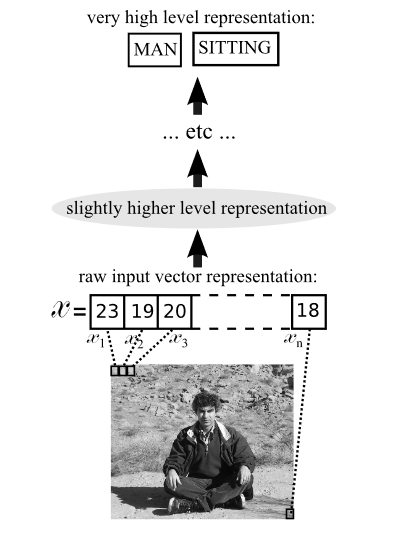
\includegraphics[width=115 mm]{images/layers-features.png}
	\caption{Minh hoạ quá trình mạng nơ-ron ``học'' từ các đặc trưng đơn giản, như các điểm ảnh, tạo thành các đặc trưng phức tạp hơn \cite{bengio2009learning}.}
	\label{fig:layers-features}
\end{figure}

Tuy nhiên, mặc dù mạng nơ-ron có càng nhiều tầng ẩn sẽ khiến cho độ chính xác trong tập huấn luyện ngày càng tăng nhưng có thể làm cho độ chính xác trong tập kiểm thử ngày càng giảm. Đây là biểu hiện của việc mô hình bị ``overfit'', đồng nghĩa với việc mô hình chỉ ``ghi nhớ'' tập huấn luyện nhưng không thể tổng quát hóa những đặc trưng đã học để tiến hành đưa ra dự đoán trên tập kiểm thử. Ngược lại, nếu mạng nơ-ron quá đơn giản, có thể có ít tầng ẩn hoặc mỗi tầng ẩn có số lượng nơ-ron ít, thì mô hình đó không đủ khả năng để rút trích ra những đặc trưng có ý nghĩa dự đoán khiến cho độ chính xác ở cả hai tập dữ liệu huấn luyện và kiểm thử đều giảm (hình \ref{fig:under-over}).

\begin{figure}[htp]
	\centering
	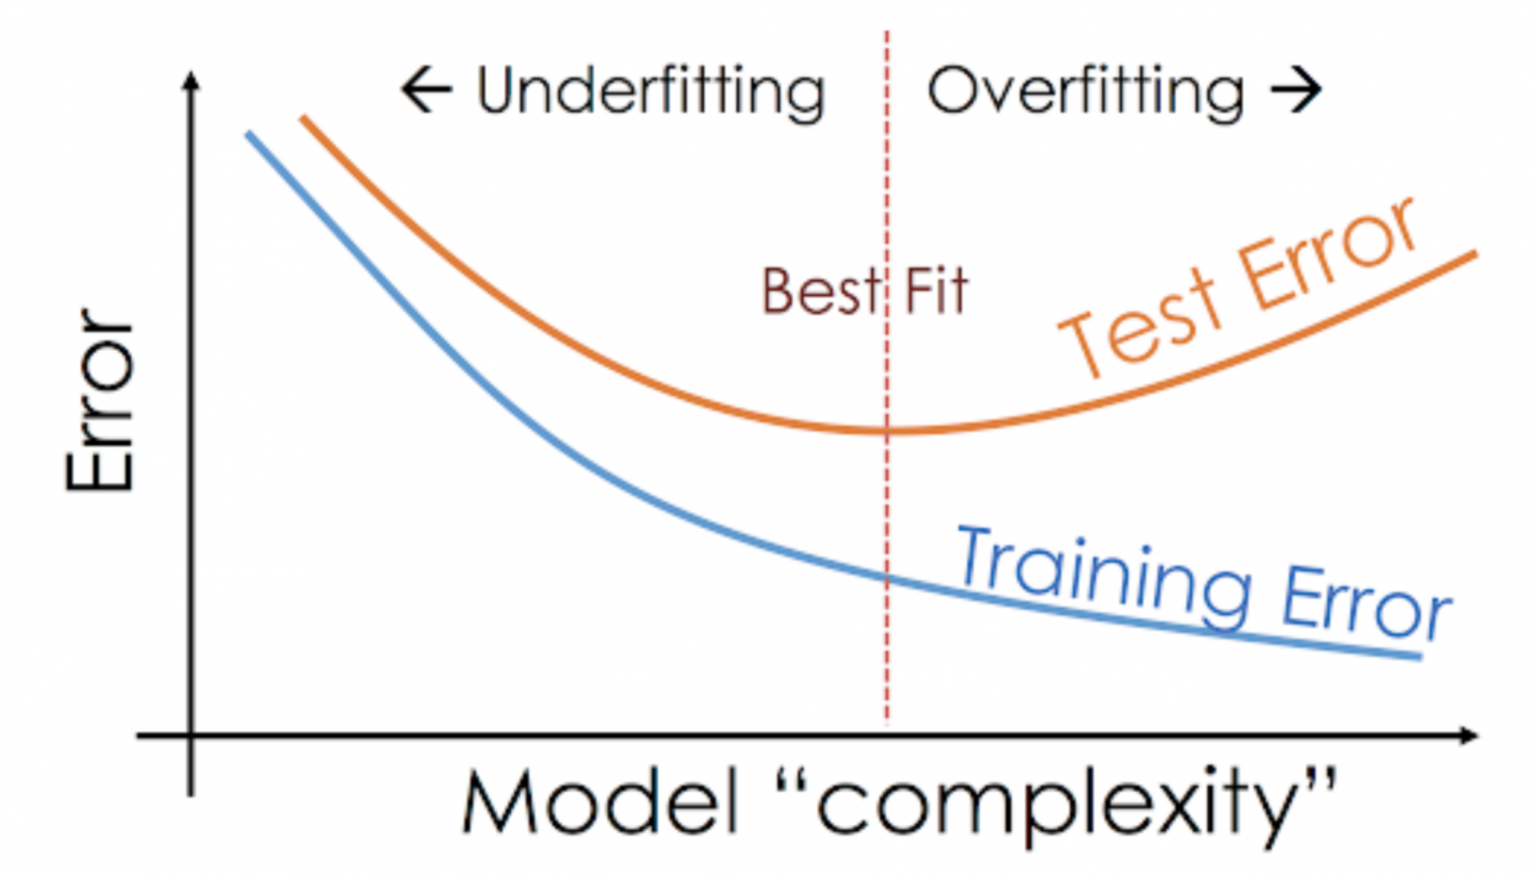
\includegraphics[width=100 mm]{images/under-over.png}
	\caption{Minh họa cho mô hình overfit và underfit. (Nguồn: \url{https://www.analyticsvidhya.com/blog/2020/02/underfitting-overfitting-best-fitting-machine-learning})}
	\label{fig:under-over}
\end{figure}

Một mạng nơ-ron nhiều tầng ẩn được xem là có khả năng tổng quát hoá tốt trên một bài toán khi sự sai khác giữa giá trị dự đoán của mạng nơ-ron và giá trị nhãn của dữ liệu ngoài tập huấn luyện là đủ nhỏ (trong bài toán huấn luyện có giám sát). Để đạt được kết quả đó, mạng nơ-ron nhiều tầng ẩn cần đi tìm một bộ trọng số phù hợp cho từng bài toán cụ thể. Việc đi tìm bộ trọng số này được thực hiện thông qua quá trình huấn luyện mạng nơ-ron nhiều tầng ẩn.

Bài toán huấn luyện mạng nơ-ron nhiều tầng ẩn nhận dữ liệu nhập là hàm chi phí nhận bộ trọng số của mạng nơ-ron nhiều tầng ẩn làm tham số. Hàm chi phí cho biết sự sai lệch giữa kết quả dự đoán của mạng nơ-ron so với giá trị đúng. Giá trị sai lệch này còn được gọi là độ lỗi. Sau quá trình huấn luyện, ta mong muốn có được một bộ trọng số của mạng nơ-ron nhiều tầng ẩn cho độ lỗi trong cả hai tập dữ liệu huấn luyện và tập dữ liệu kiểm thử là đủ nhỏ.

\begin{figure}[htp]
	\centering
	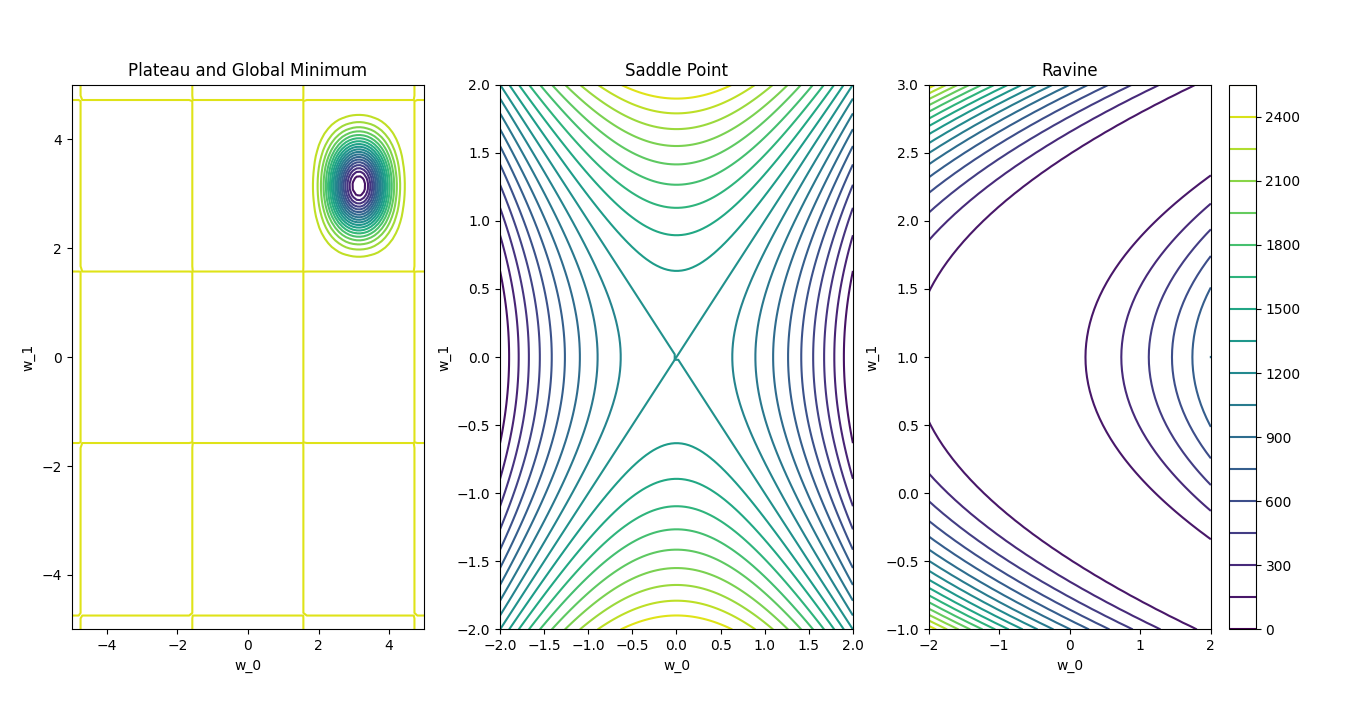
\includegraphics[width=120 mm]{images/cricial-point-contour.png}
	\caption{Đồ thị contour cho những điểm critical point: vùng bằng phẳng có một cực tiểu (trái), điểm yên ngựa (giữa), vùng rãnh hẹp (phải).}
	\label{fig:cricial-point-contour}
\end{figure}

Việc huấn luyện, hay tối ưu hoá mạng nơ-ron có thể hiểu là quá trình đi tìm cực tiểu của hàm chi phí bằng cách thay đổi giá trị của bộ trọng số. Từ đó, ta cũng có thể hiểu quá trình tối ưu hóa mạng nơ-ron là quá trình di chuyển trong bề mặt lỗi (hình \ref{fig:resnet-loss}) dựa trên hướng của véc-tơ đạo hàm riêng, còn được gọi là gradient. Tuy nhiên, việc di chuyển trong bề mặt lỗi gặp nhiều khó khăn. Li Hao và cộng sự \cite{li2018visualizing} cho thấy rằng sự phức tạp của bề mặt lỗi ngày càng tăng khi số tầng ẩn trọng mạng nơ-ron ngày càng tăng. Sự hỗn loạn này được cấu thành từ nhiều ``critical point'' (``critical point'' là những điểm có gradient bằng 0 như cực tiểu địa phương, điểm yên ngựa) hợp với các vùng bằng phẳng, và vùng rãnh hẹp (hình \ref{fig:cricial-point-contour}).

\begin{figure}[htp]
	\centering
	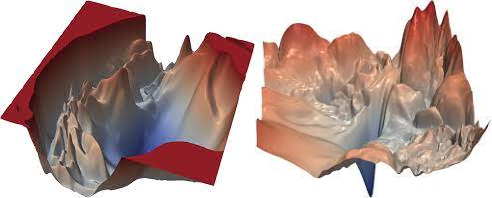
\includegraphics[width=120 mm]{images/resnet-loss.png}
	\caption{Bề mặt lỗi của mô hình ResNet-110 (trái) và bề mặt lỗi của mô hình ResNet-56 (phải) \cite{li2018visualizing}.}
	\label{fig:resnet-loss}
\end{figure}

Các điểm cực tiểu địa phương từng được xem như là nguyên nhân chính gây ra sự khó khăn trong việc tối ưu hoá mạng nơ-ron có nhiều tầng ẩn, nhưng nghiên cứu của Quynh Nguyen và Matthias Hein \cite{nguyen2017thelosssurface} đã chỉ ra rằng việc đi tìm cực tiểu toàn cục có thể mất nhiều thời gian nhưng cho hiệu quả không đáng kể. Yann N. Dauphin cũng cho rằng khi số lượng tầng ẩn quá lớn thì phần lớn các điểm critical point sẽ là điểm yên ngựa, và các điểm cực tiểu tìm được đều có độ lỗi ngang với cực tiểu toàn cục. Hơn nữa, các điểm yên ngựa thường được bao bọc bởi một vùng gần như bằng phẳng, là vùng mà tại đó đạo hàm gần bằng 0, làm chậm tốc độ của đa số các thuật toán tối ưu thường được sử dụng hiện nay.

\begin{figure}[htp]
	\centering
	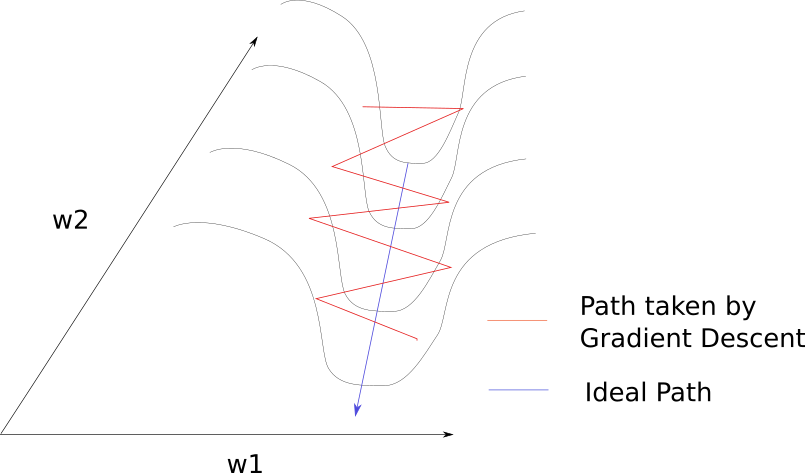
\includegraphics[width=100 mm]{images/valley.png}
	\caption{Minh họa cho hướng đi của gradient trong trường hợp di chuyển trong rãnh hẹp. (Nguồn: \url{https://blog.paperspace.com/intro-to-optimization-momentum-rmsprop-adam/})}
	\label{fig:valley}
\end{figure}

Ngoài các điểm yên ngựa, bề mặt lỗi còn đặc trưng bởi độ cong tại mỗi hướng tương ứng với một trọng số của mạng nơ-ron nhiều tầng ẩn. Một hướng có độ cong thấp (low-curvature, như hướng $w_2$ trong hình \ref{fig:valley}) đồng nghĩa với gradient sẽ ít thay đổi và ngược lại, một hướng có độ cong cao (high-curvature, như hướng $w_1$ trong hình \ref{fig:valley}) sẽ có gradient thay đổi nhiều. Vùng được đồng thời tạo bởi các hướng có độ cong cao và độ cong thấp được gọi là vùng rãnh hẹp. Các vùng này được tạo ra do ảnh hưởng của các trọng số $w_1$ và $w_2$ lên độ lỗi là không giống nhau. Một $w_1$ có giá trị gấp 10 lần giá trị của $w_2$ sẽ cho tín hiệu của các nơ-ron được liên kết bằng $w_1$ ảnh hưởng lên độ lỗi gấp 10 lần tín hiệu của các nơ-ron được liên kết bằng $w_2$, dẫn đến độ cong theo hướng $w_1$ sẽ cao hơn độ cong theo hướng $w_2$ gấp 10 lần. Sự cách biệt lớn trong độ lớn của các giá trị trọng số này tạo ra vùng rãnh hẹp. Hiện tượng này thường xuyên xảy ra trong mạng nơ-ron do tín hiệu của các nơ-ron khác nhau có mức độ ảnh hưởng khác nhau đến quá trình dự đoán, và càng nghiêm trọng hơn trong các mạng nơ-ron nhiều tầng ẩn.

Phương pháp đầu tiên được dùng trong huấn luyện mạng nơ-ron thực hiện bước từng bước nhỏ từ một điểm bất kỳ theo hướng ngược lại với hướng có độ tăng lớn nhất, hướng của véc-tơ đạo hàm riêng gradient, tìm đến điểm cho độ lỗi nhỏ hơn được gọi là ``Gradient Descent'' (GD). Tuy nhiên, phương pháp này tốn nhiều thời gian tính toán véc-tơ gradient tại điểm hiện tại. Các đạo hàm riêng theo từng trọng số trong gradient có được từ việc lấy đạo hàm của trung bình độ lỗi trên toàn bộ điểm dữ liệu. Với kích thước tập dữ liệu cần cho huấn luyện mạng nơ-ron nhiều tầng ẩn càng lớn thì việc tính toán gradient tại mỗi bước lại càng mất nhiều thời gian. Để cải thiện vấn đề này, một phương pháp khác không sử dụng toàn bộ điểm dữ liệu để thực hiện một bước cập nhật, thay vào đó, chỉ một tập con lấy ngẫu nhiên được sử dụng để tính véc-tơ gradient tại mỗi bước. Phương pháp này được gọi là ``Stochastic Gradient Descent'' (SGD). Vì thực hiện tính toán trên một tập con dữ liệu nên hướng gradient của SGD chỉ là một xấp xỉ của hướng gradient thật của bề mặt lỗi có độ sai số tỉ lệ nghịch với kích thước tập con.

Tuy nhiên, SGD thực hiện một bước nhảy tỉ lệ với độ lớn của gradient nên gặp khó khăn khi di chuyển trong các vùng rãnh hẹp và vùng có độ nghiêng nhỏ. Trong những vùng này, ta mong muốn độ lớn bước cập nhật tỉ lệ nghịch với độ lớn của gradient. Vì vùng có độ lớn gradient nhỏ thì một bước đi dài sẽ giúp giảm thời gian di chuyển trong khi những vùng có gradient lớn cần bước những bước nhỏ hơn. Sự điều chỉnh này trong bước cập nhật của SGD cho ta thuật toán ``SGD với Momentum'', hay ``Momentum''. Thuật toán Momentum cập nhật trọng số dựa trên gradient của bước hiện tại và gradient của những bước cập nhật gần nhất. Từ đó, một lượng ``quán tính" được thêm vào giúp triệt tiêu các hướng có độ cong cao và cho phép một bước cập nhật lớn hơn tại hướng có độ dốc thấp. Bước cải tiến này không chỉ giúp thuật toán Momentum thực hiện những bước cập nhật có ý nghĩa trong vùng rãnh hẹp và vùng có độ nghiêng nhỏ mà còn giúp xấp xỉ gradient trong SGD gần hơn với gradient thật của bề mặt lỗi từ đó tăng độ chính xác trong hướng di chuyển của thuật toán.

Thuật toán SGD với Momentum giúp cải thiện tốc độ huấn luyện mạng nơ-ron đáng kể và vẫn được sử dụng trong một số mạng nơ-ron nhiều tầng ẩn hiện nay. Mặc dù vậy thuật toán vẫn chưa giải quyết được các khó khăn vì lượng "quán tính" được thêm vào không có nhiều hiệu quả trong những vùng rãnh hẹp mà độ lớn của đạo hàm riêng tại mỗi hướng cập nhật rất khác nhau. Richard S. Sutton cho rằng để có được một bước cập nhật có hiệu quả thì tỉ lệ học cần phải được thay đổi ứng với độ cong của từng hướng\cite{sutton1986two}. Đây là một trong những lý do các phương pháp bậc hai được sử dụng. Các phương pháp bậc hai là những phương pháp sử dụng ma trận Hessian — là ma trận đạo hàm riêng bậc hai theo từng cặp hướng — để ước lượng độ cong tại một điểm trên bề mặt lỗi. Từ các ước lượng bậc hai này mà các phương pháp bậc hai cho bước cập nhật tốt hơn các phương pháp chỉ sử dụng gradient.

Mặc dù phương pháp bậc hai cho các bước cập nhật tối ưu nhưng có hai nguyên nhân dẫn tới các phương pháp này ít được sử dụng trong huấn luyện mạng nơ-ron nhiều tầng ẩn hiện nay. Đầu tiên, việc sử dụng các xấp xỉ bậc hai dẫn đến dao động tại vùng gần cực tiểu kéo dài thời gian huấn luyện và có khả năng không thể hội tụ. Khó khăn thứ hai đến từ việc tính toán ma trận Hessian đòi hỏi nhiều chi phí tính toán và tiêu tốn bộ nhớ cấp số mũ với số lượng trọng số của mạng. Đối với các mạng nơ-ron nhiều tầng ẩn có số trọng số có thể lên tới hàng tỷ thì đây là điều bất khả thi. Vì vậy, một số phương pháp bậc nhất thực hiện xấp xỉ ma trận Hessian thông qua gradient bậc nhất. Đây là ý tưởng chính của các thuật toán sử dụng tỉ lệ học thích ứng. Các thuật toán này điều chỉnh tỉ lệ học tại từng hường bằng cách sử dụng bình phương đạo hàm riêng bậc nhất của trọng số tương ứng. Vì mỗi trọng số được cập nhật một lượng riêng lẻ nên véc-tơ đạo hàm riêng là một hình chiếu của véc-tơ gradient trên trục trọng số tương ứng. Độ dài của véc-tơ hình chiếu sẽ lớn nhất khi véc-tơ gradient song song với trục và giảm dần khi véc-tơ gradient càng vuông góc với trục. Chính vì lý do đó mà các thuật toán sử dụng tỉ lệ học thích ứng gặp nhiều khó khăn khi các hướng tối ưu không phải là hướng song song với trục trọng số.

Lấy ý tưởng từ những phương pháp trên, Diederik P. Kingma và Jimmy Lei Ba đã đề xuất một thuật toán tối ưu bậc nhất cho mạng nơ-ron nhiều tầng ẩn với tốc độ cao hơn so với hầu hết những thuật toán trước đó \cite{kingma2014adam}. Công trình này, ``Adam, A Method for Stochastic Optimization'', được công bố tại hội nghị ``International Conference on Learning Representation 2015''. Ý tưởng của thuật toán là kết hợp hai hướng tiếp cận trước đó: (1) sử dụng quán tính để tăng tốc và giảm dao động, và (2) thích ứng tỉ lệ học cho từng trọng số. Thuật toán Adam sử dụng trung bình chạy để tích tụ quán tính kết hợp với phương pháp xấp xỉ ma trận Hessian của phương pháp tỉ lệ học thích ứng. Sự kết hợp này cho phép thực hiện các bước cập nhật tốt hơn tại vùng có độ lớn đạo hàm riêng trên mỗi hướng rất khác nhau. Đồng thời cũng cải thiện độ lớn của bước cập nhật khi véc-tơ gradient không song song với trục trọng số. Ngoài ra, Adam còn thực hiện ``bias-correction'' giúp thuật toán không bị ``bias'' về giá trị khởi tạo cho phép thực hiện các bước cập nhật tốt hơn ngay những bước đầu tiên. Trong khóa luận này, chúng tôi tìm hiểu và cài đặt lại thuật toán Adam cùng với các thuật toán liên quan. Chúng tôi cũng thực hiện thêm các thí nghiệm nhằm phân tích và làm rõ cách mỗi phương pháp giải quyết các khó khăn trong việc huấn luyện mạng nơ-ron nhiều tầng ẩn. Ngoài ra, chúng tôi cũng sử dụng tính toán song song trên GPU để tăng tốc độ xử lí cho các thí nghiệm.

Phần còn lại của khóa luận được trình bày như sau:

\begin{itemize}
	\item Chương 2 giới thiệu sơ lược về mạng nơ-ron nhiều tầng ẩn và quá trình huấn luyện, cũng như nguyên lý của thuật toán Gradient Descent.
	\item Chương 3 trình bày về thuật toán Adam và các thuật toán nền tảng. Chương này là phần chính của khóa luận.
	\item Chương 4 trình bày về các thí nghiệm về nguyên lý cũng như thực tiễn để phân tích các tính chất của thuật toán Adam.
	\item Cuối cùng, chương 5 trình bày kết luận và hướng phát triển.
\end{itemize}
